\documentclass[tikz, margin=2mm, convert={density=300,size=1920x1080,outext=.png}]{standalone}

\pgfdeclarelayer{last}
\pgfdeclarelayer{middle-3}
\pgfdeclarelayer{middle-2}
\pgfdeclarelayer{middle-1}
\pgfdeclarelayer{second}
\pgfdeclarelayer{first}
\pgfsetlayers{last,middle-3,middle-2,middle-1,second,first,main}


% \pgfdeclarelayer{x2-m1}
% \pgfdeclarelayer{x2-m2}
% \pgfdeclarelayer{x2-m3}
% \pgfdeclarelayer{x3}
% \pgfdeclarelayer{x4}
% \pgfdeclarelayer{x1}
% \pgfsetlayers{x4,x3,x2-m1,x2-m2,x2-m3,x1,main}  % set the order of the layers (main is the standard layer)

\tikzset{
    % neurons
    neuron/.style={
        circle,
        draw=none,
        shading=ball,
        minimum size=1cm
    },
    neuron-missingvert/.style={
        draw=none,
        scale=3,
        text height=0.3333cm,
        fill=none,
        execute at begin node=\color{black}$\vdots$
    },
    neuron-missingdiag/.style={
        draw=none,
        scale=3,
        text height=0.3333cm,
        execute at begin node=\color{black}$\ddots$
    },
    neuron-blank/.style={
        draw=none,
    },
    neuron-missing/.style={
        draw=none,
        scale=3,
        text height=0.25cm,
        execute at begin node=\color{black}$\cdotp$
    },
    % arrows
    first-layer/.style={
        line width=2pt,
        color=black!80,
        opacity=.8
    },
    second-layer/.style={
        line width=2pt,
        opacity=.4
    },
    last-layer/.style={
        line width=2pt,
        opacity=.1
    }
}

\begin{document}
    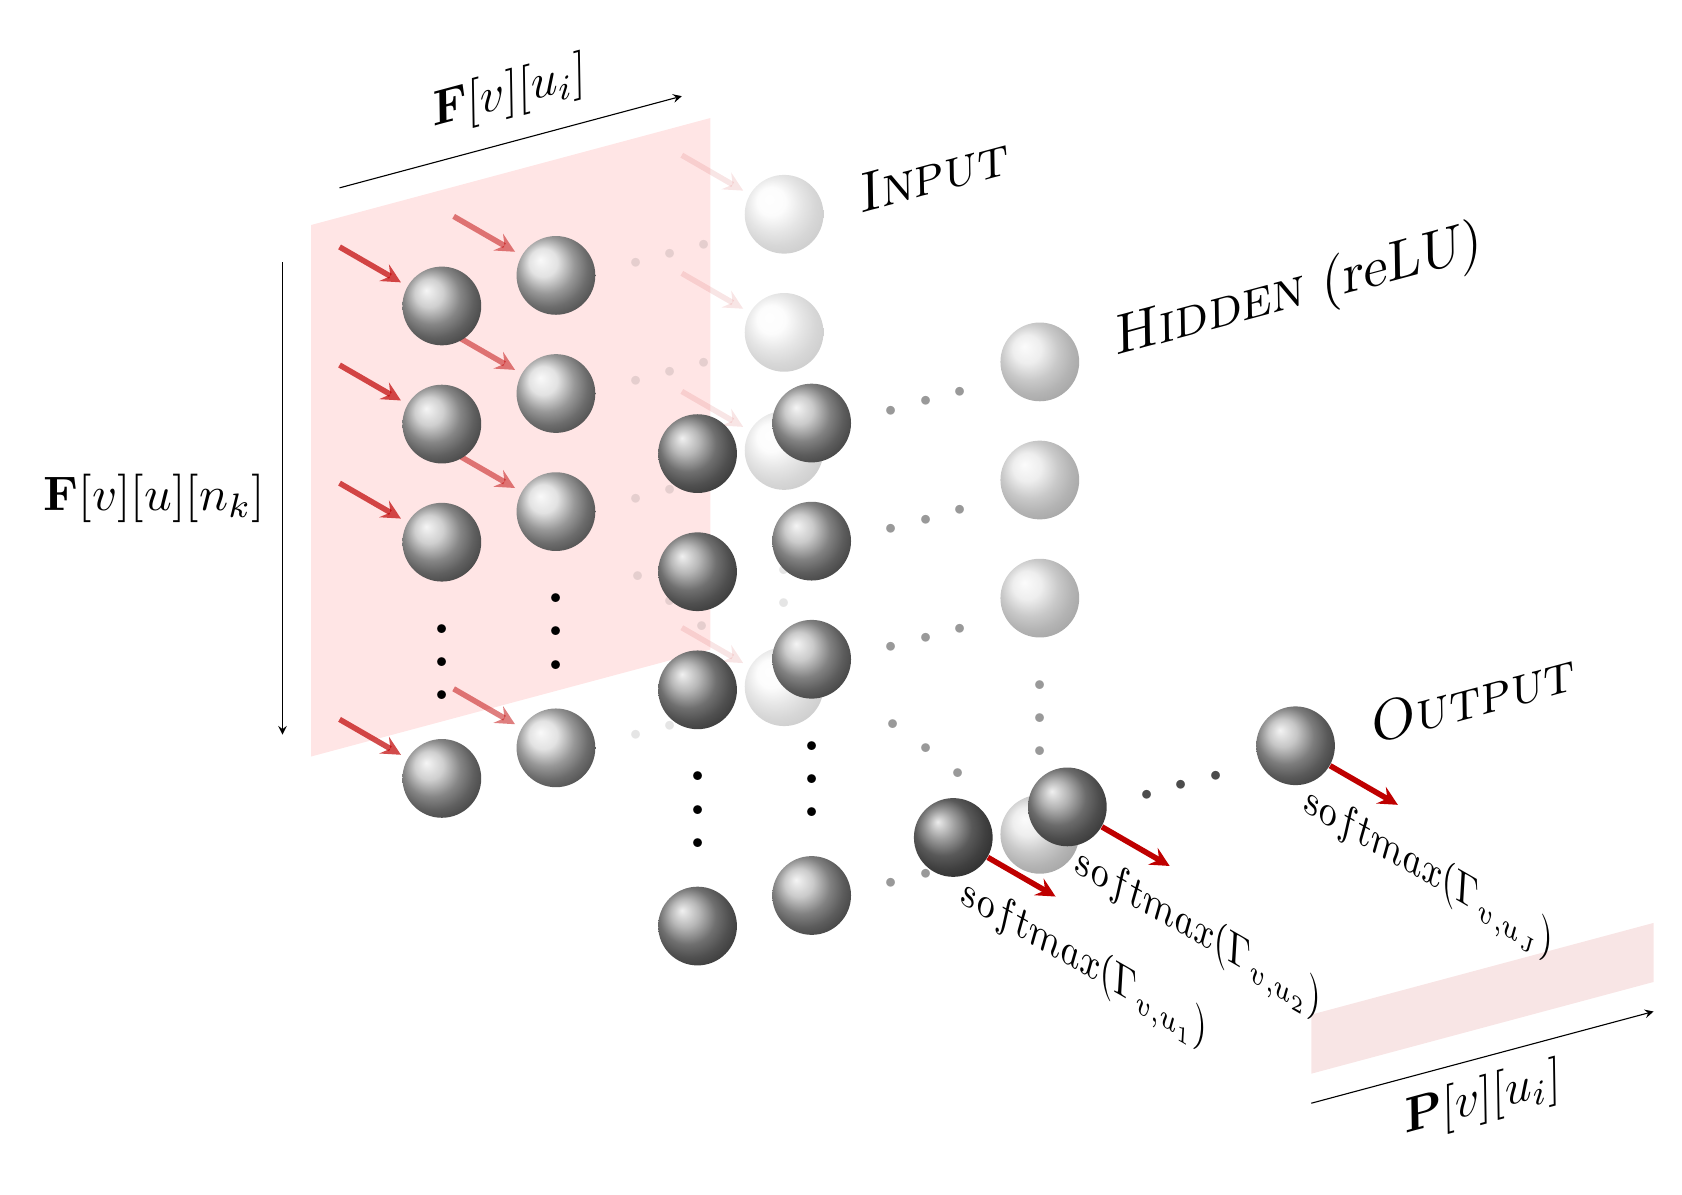
\begin{tikzpicture}[x=(15:1.5cm), y=(90:1.5cm), z=(330:1.5cm), >=stealth]

        \begin{pgfonlayer}{last}
            % input dataset
            \fill[red, opacity=.1] (-.25, -.75, -1) -- (3.25, -.75, -1) -- (3.25, -5.25, -1) -- (-.25, -5.25, -1) --cycle;
            % draw nodes
            \foreach \m [count=\y] in {1, 2, 3, 4, 5} {
                \ifnum\m=4
                    \node [neuron-missingvert, opacity=.1] at (3, -\y, 0) {};
                \else
                    \node [neuron, ball color=gray!10, opacity=.3] (input-3\m) at (3, -\y, 0) {};
                    \draw[->, line width=2pt, red!75!black, opacity=.1] (3, -\y, -1) -- ++(0, 0, .6);
                \fi
                
            }
            \foreach \m [count=\y] in {1, 2, 3, 4, 5} {
                \ifnum\m=4
                    \node [neuron-missingvert, opacity=.4] at (3, -\y, 2.5) {};
                \else
                    \node [neuron, ball color=gray!35, opacity=.5] (hidden-3\m) at (3, -\y, 2.5) {};
                \fi
            }
            \node [neuron, ball color=gray!60] (output-3) at (3, -3, 5) {};

            % draw edges
%            \foreach \m in {1, 2, 3, 5}
%                \draw[->, last-layer] (input-3\m) -- (output-3);
        \end{pgfonlayer}

        \begin{pgfonlayer}{middle-3}
            \foreach \m [count=\y] in {1, 2, 3, 4, 5} {
                \ifnum\m=4
                    \node [neuron-blank] at (2.3, -\y, 0) {};
                \else
                    \node [neuron-missing, opacity=.1] at (2.3, -\y, 0) {};
                \fi
            }
            \foreach \m [count=\y] in {1, 2, 3, 4, 5} {
                \ifnum\m=4
                    \node [neuron-blank] at (2.3, -\y, 2.5) {};
                \else
                    \node [neuron-missing, opacity=.4] at (2.3, -\y, 2.5) {};
                \fi
            }
            \node [neuron-missing, opacity=.7] at (2.3, -3, 5) {};
        \end{pgfonlayer}

        \begin{pgfonlayer}{middle-2}
            \foreach \m [count=\y] in {1, 2, 3, 4, 5} {
                \ifnum\m=4
                    \node [neuron-missingdiag, opacity=.1] at (2, -\y, 0) {};
                \else
                    \node [neuron-missing, opacity=.1] at (2, -\y, 0) {};
                \fi
            }
            \foreach \m [count=\y] in {1, 2, 3, 4, 5} {
                \ifnum\m=4
                    \node [neuron-missingdiag, opacity=.4] at (2, -\y, 2.5) {};
                \else
                    \node [neuron-missing, opacity=.4] at (2, -\y, 2.5) {};
                \fi
            }
            \node [neuron-missing, opacity=.7] at (2, -3, 5) {};
        \end{pgfonlayer}

        \begin{pgfonlayer}{middle-1}
            \foreach \m [count=\y] in {1, 2, 3, 4, 5} {
                \ifnum\m=4
                    \node [neuron-blank] at (1.7, -\y, 0) {};
                \else
                    \node [neuron-missing, opacity=.1] at (1.7, -\y, 0) {};
                \fi
            }
            \foreach \m [count=\y] in {1, 2, 3, 4, 5} {
                \ifnum\m=4
                    \node [neuron-blank] at (1.7, -\y, 2.5) {};
                \else
                    \node [neuron-missing, opacity=.4] at (1.7, -\y, 2.5) {};
                \fi
            }
            \node [neuron-missing, opacity=.7] at (1.7, -3, 5) {};
        \end{pgfonlayer}

        \begin{pgfonlayer}{second}
            % draw nodes
            \foreach \m [count=\y] in {1, 2, 3, 4, 5} {
                \ifnum\m=4
                    \node [neuron-missingvert] at (1, -\y, 0) {};
                \else
                    \node [neuron, ball color=gray!30] (input-2\m) at (1, -\y, 0) {};
                    \draw[->, line width=2pt, red!75!black, opacity=.5] (1, -\y, -1) -- ++(0, 0, .6);
                \fi
            }
            \foreach \m [count=\y] in {1, 2, 3, 4, 5} {
                \ifnum\m=4
                    \node [neuron-missingvert] at (1, -\y, 2.5) {};
                \else
                    \node [neuron, ball color=gray!55] (hidden-2\m) at (1, -\y, 2.5) {};
                \fi
            }
            \node [neuron, ball color=gray!80] (output-2) at (1, -3, 5) {};

            % draw edges
%            \foreach \m in {1, 2, 3, 5}
%                \draw[->, second-layer] (input-2\m) -- (output-2);
        \end{pgfonlayer}

        \begin{pgfonlayer}{first}
            % draw nodes
            \foreach \m [count=\y] in {1, 2, 3, 4, 5} {
                \ifnum\m=4
                    \node [neuron-missingvert, color=gray!50] at (0, -\y, 0) {};
                \else
                    \node [neuron, ball color=gray!50] (input-1\m) at (0, -\y, 0) {};
                    \draw[->, line width=2pt, red!75!black, opacity=.7] (0, -\y, -1) -- ++(0, 0, .6);
                \fi
            }
            \foreach \m [count=\y] in {1, 2, 3, 4, 5} {
                \ifnum\m=4
                    \node [neuron-missingvert, color=gray!75] at (0, -\y, 2.5) {};
                \else
                    \node [neuron, ball color=gray!75] (hidden-1\m) at (0, -\y, 2.5) {};
                \fi
            }
            \node [neuron/.try, ball color=gray] (output-1) at (0, -3, 5) {};

            % draw edges
%            \foreach \m in {1, 2, 3, 5}
%                \draw[->, first-layer] (input-1\m) -- (output-1);
        \end{pgfonlayer}
        
        % output
        \fill[red!75!black, opacity=.1] (0, -2.75, 8.5) -- (3, -2.75, 8.5) -- (3, -3.25, 8.5) -- (0, -3.25, 8.5) -- cycle;

        % markings
        \draw [->] (-.5, -1, -1)  -- (-.5, -5, -1)   node [midway, left, scale=1.75] {$\mathbf{F}[v][u][n_k]$};
        
        \draw [->] (0, -.5, -1)  -- (3, -.5, -1)   node [midway, above=2pt, rotate=15, xslant=.25, scale=1.75] {$\mathbf{F}[v][u_i]$};
        
        \foreach \l [count=\i] in {1, 2, J}
        \draw [->, line width=2pt, red!75!black] (output-\i) -- ++(0, 0, 1) node [below=-5pt, right=-40pt, black, rotate=330, xslant=-.5, scale=1.5] {$softmax(\Gamma_{v, u_\l})$};
        
        % names
        \node [align=center, right, rotate=15, xslant=.25, scale=2] at (3.5, -1, 0) {\textsc{Input}};
        \node [align=center, right, rotate=15, xslant=.25, scale=2] at (3.5, -1, 2.5) {\textsc{Hidden} (reLU)};
        \node [align=center, right, rotate=15, xslant=.25, scale=2] at (3.5, -3, 5) {\textsc{Output}};
        \draw [->] (0, -3.5, 8.5) -- (3, -3.5, 8.5) node [midway, below, rotate=15, xslant=.25, scale=1.75] {$\mathbf{P}[v][u_i]$};
    \end{tikzpicture}
\end{document}
